\chapter{Experiments}

This chapter evaluates the main contributions described in the previous chapters. It examines the user-feedback threshold refinement workflow and presents visual case studies on the ECG and Weather datasets.

\section{Experiment Setup}
The experiment was conducted on a local Windows laptop. The machine uses an Intel(R) Core(TM) i7-10510U CPU @ 1.80GHz with 8 logical processors and 16 GB of physical memory. The operating system is Windows 11, 64-bit. The system uses Python 3.9.0 as the runtime environment, and the main Python dependencies include Flask, NumPy, pandas, SciPy, scikit-learn, STUMPY, and TSB-UAD.


\section{Datasets}
\fei{Separate each dataset description to its own paragraph for easier readability.}
\reply{Separate the dataset description into three paragraphs, different paragraphs correspond to different datasets.}{}

\textcolor{blue}{Three time-series datasets were used to evaluate the system: ECG, Elec, and Weather. These datasets include anomalies and concept drifts.}

\textcolor{blue}{The ECG dataset is a periodic electrocardiogram dataset from the TSB-UAD benchmark suite. It contains approximately 230K time points and labeled anomalies related to premature ventricular contractions \citep{park2025andri,paparrizos2022tsbuad}. Abrupt and recurrent drift were injected by transitioning between selected ECG patterns. This setting is useful for evaluating whether a detector can avoid treating a change in normal ECG pattern as an anomaly.}

\textcolor{blue}{The Elec dataset describes electricity usage in New South Wales, Australia. It contains approximately 45K time points collected over 2.5 years, with concept drift caused by weekday-to-weekend changes and seasonal usage variation \citep{park2025andri,bifet2010moa}. Anomalies were injected into the series by modifying selected values. This dataset represents energy-consumption data where normal behavior can change because of calendar and seasonal effects.}

\textcolor{blue}{The Weather dataset contains hourly, geographically aggregated temperature records of European countries from 2017 to 2020. It contains approximately 26K time points and includes naturally occurring gradual concept drift caused by seasonal changes \citep{park2025andri,gelaro2017merra2}. The Weather dataset provides a more natural example of gradual drift in real-world time-series data.}

\textcolor{blue}{Among these three data sets, the proportion of anomalies in the ECG data set is 5\%, while the proportions of anomalies in the other two data sets, namely Elec and Weather, are both 10\%.}


Three time-series datasets were used to evaluate the system: ECG, Elec, and Weather. These datasets include anomalies and concept drifts. The ECG dataset is a periodic electrocardiogram dataset from the TSB-UAD benchmark suite. It contains approximately 230K time points and labeled anomalies related to premature ventricular contractions \citep{park2025andri,paparrizos2022tsbuad}. Abrupt and recurrent drift were injected by transitioning between selected ECG patterns. This setting is useful for evaluating whether a detector can avoid treating a change in normal ECG pattern as an anomaly. The Elec dataset describes electricity usage in New South Wales, Australia. It contains approximately 45K time points collected over 2.5 years, with concept drift caused by weekday-to-weekend changes and seasonal usage variation \citep{park2025andri,bifet2010moa}. Anomalies were injected into the series by modifying selected values. This dataset represents energy-consumption data where normal behavior can change because of calendar and seasonal effects. The Weather dataset contains hourly, geographically aggregated temperature records of European countries from 2017 to 2020. It contains approximately 26K time points and includes naturally occurring gradual concept drift caused by seasonal changes \citep{park2025andri,gelaro2017merra2}. The Weather dataset provides a more natural example of gradual drift in real-world time-series data. Among these three data sets, the proportion of anomalies in the ECG data set is 5\%, while the proportions of anomalies in the other two data sets, namely Elec and Weather, are both 10\%.


\section{Baselines}

% \fei{Include references to each baseline, GitHub source for data and code.}

\noindent To evaluate the ECG results, AnDri was compared with three baseline anomaly detection methods: NormA, SAND, and DAMP. The ECG dataset is taken from the public TSB-UAD benchmark repository,\footnote{\url{https://github.com/TheDatumOrg/TSB-UAD}} while the AnomDrift is implemented in the project repository.\footnote{\url{https://github.com/ZeeChee-Guo/AndriDemo}} For the baseline implementations, SAND and DAMP are integrated through publicly available benchmark or project code. NormA is treated separately because its source code is not directly included in the TSB-UAD repository used in this project; access to the NormA implementation needs to be requested from the original authors.


\section{Evaluation Metrics}


The evaluation compares the final predicted anomaly labels with the ground-truth labels in the datasets.

After the adaptive thresholding step, each method has a final threshold. The anomaly score of each point is compared with this threshold to generate a binary prediction. For NormA, SAND, and DAMP, one global threshold is used:
\[\hat{y}_i = 1 \quad \text{if} \quad s_i > \theta.\]
For AnDri, the threshold is associated with the normal pattern assigned to the point:
\[ \hat{y}_i = 1 \quad \text{if} \quad s_i > \theta_{m_i}.\]
Otherwise, \(\hat{y}_i = 0\). The predicted labels \(\hat{y}_i\) are then compared with the ground-truth labels \(y_i = \textbf{GroundTruth[i]}\) to calculate precision, recall, and F1-score.

The prediction results are evaluated using precision, recall, and F1-score. Let TP denote true positives, FP denote false positives, and FN denote false negatives. TP is the number of anomaly-labeled points correctly detected as anomalies. FP is the number of normal points incorrectly detected as anomalies. FN is the number of anomaly-labeled points missed by the method.

\[Precision = \frac{TP}{TP + FP}\]

\[Recall = \frac{TP}{TP + FN}\]

\[F1 = \frac{2 \times Precision \times Recall}{Precision + Recall}\]

Precision measures how many detected anomalies are correct. Recall measures how many true anomalies are successfully detected. F1-score combines precision and recall into one value. The experiments also report AUC-ROC. A higher AUC indicates better overall separation between anomalous and normal regions.



\section{User-Feedback Threshold Refinement Results and Analysis}

This section evaluates the feedback efficiency of the threshold-refinement process. Specifically, this chapter explores how user feedback can enhance the F1-score of anomaly detection.

The initial threshold is determined by the user-specified anomaly proportion $\alpha$. Specifically, the threshold is selected such that the top-$\alpha$ highest-scoring points are classified as anomalies. For example, when $\alpha=5\%$, the threshold is chosen so that the 5\% of points with the highest anomaly scores are labeled as anomalies, while the remaining 95\% are labeled as normal.

To evaluate feedback efficiency, ground-truth labels are used to simulate correct user feedback. The experiment investigates how detection performance changes as the amount of available feedback increases.

The user-labeled anomaly ratio is varied from 0\% to 100\%. A ratio of 0\% represents the fully automatic baseline, where no user feedback is provided and the final labels are generated directly using the initial threshold determined by $\alpha$ . A ratio of 5\% means that only 5\% of the ground-truth anomaly points within the training set are provided as user-confirmed anomalies, while the remaining anomaly points remain unlabeled. For each ratio, anomaly points are randomly sampled from the training set, and the experiment is repeated 30 times. The reported curves show the average F1-score across the 30 runs.

\begin{figure}[H]
\centering
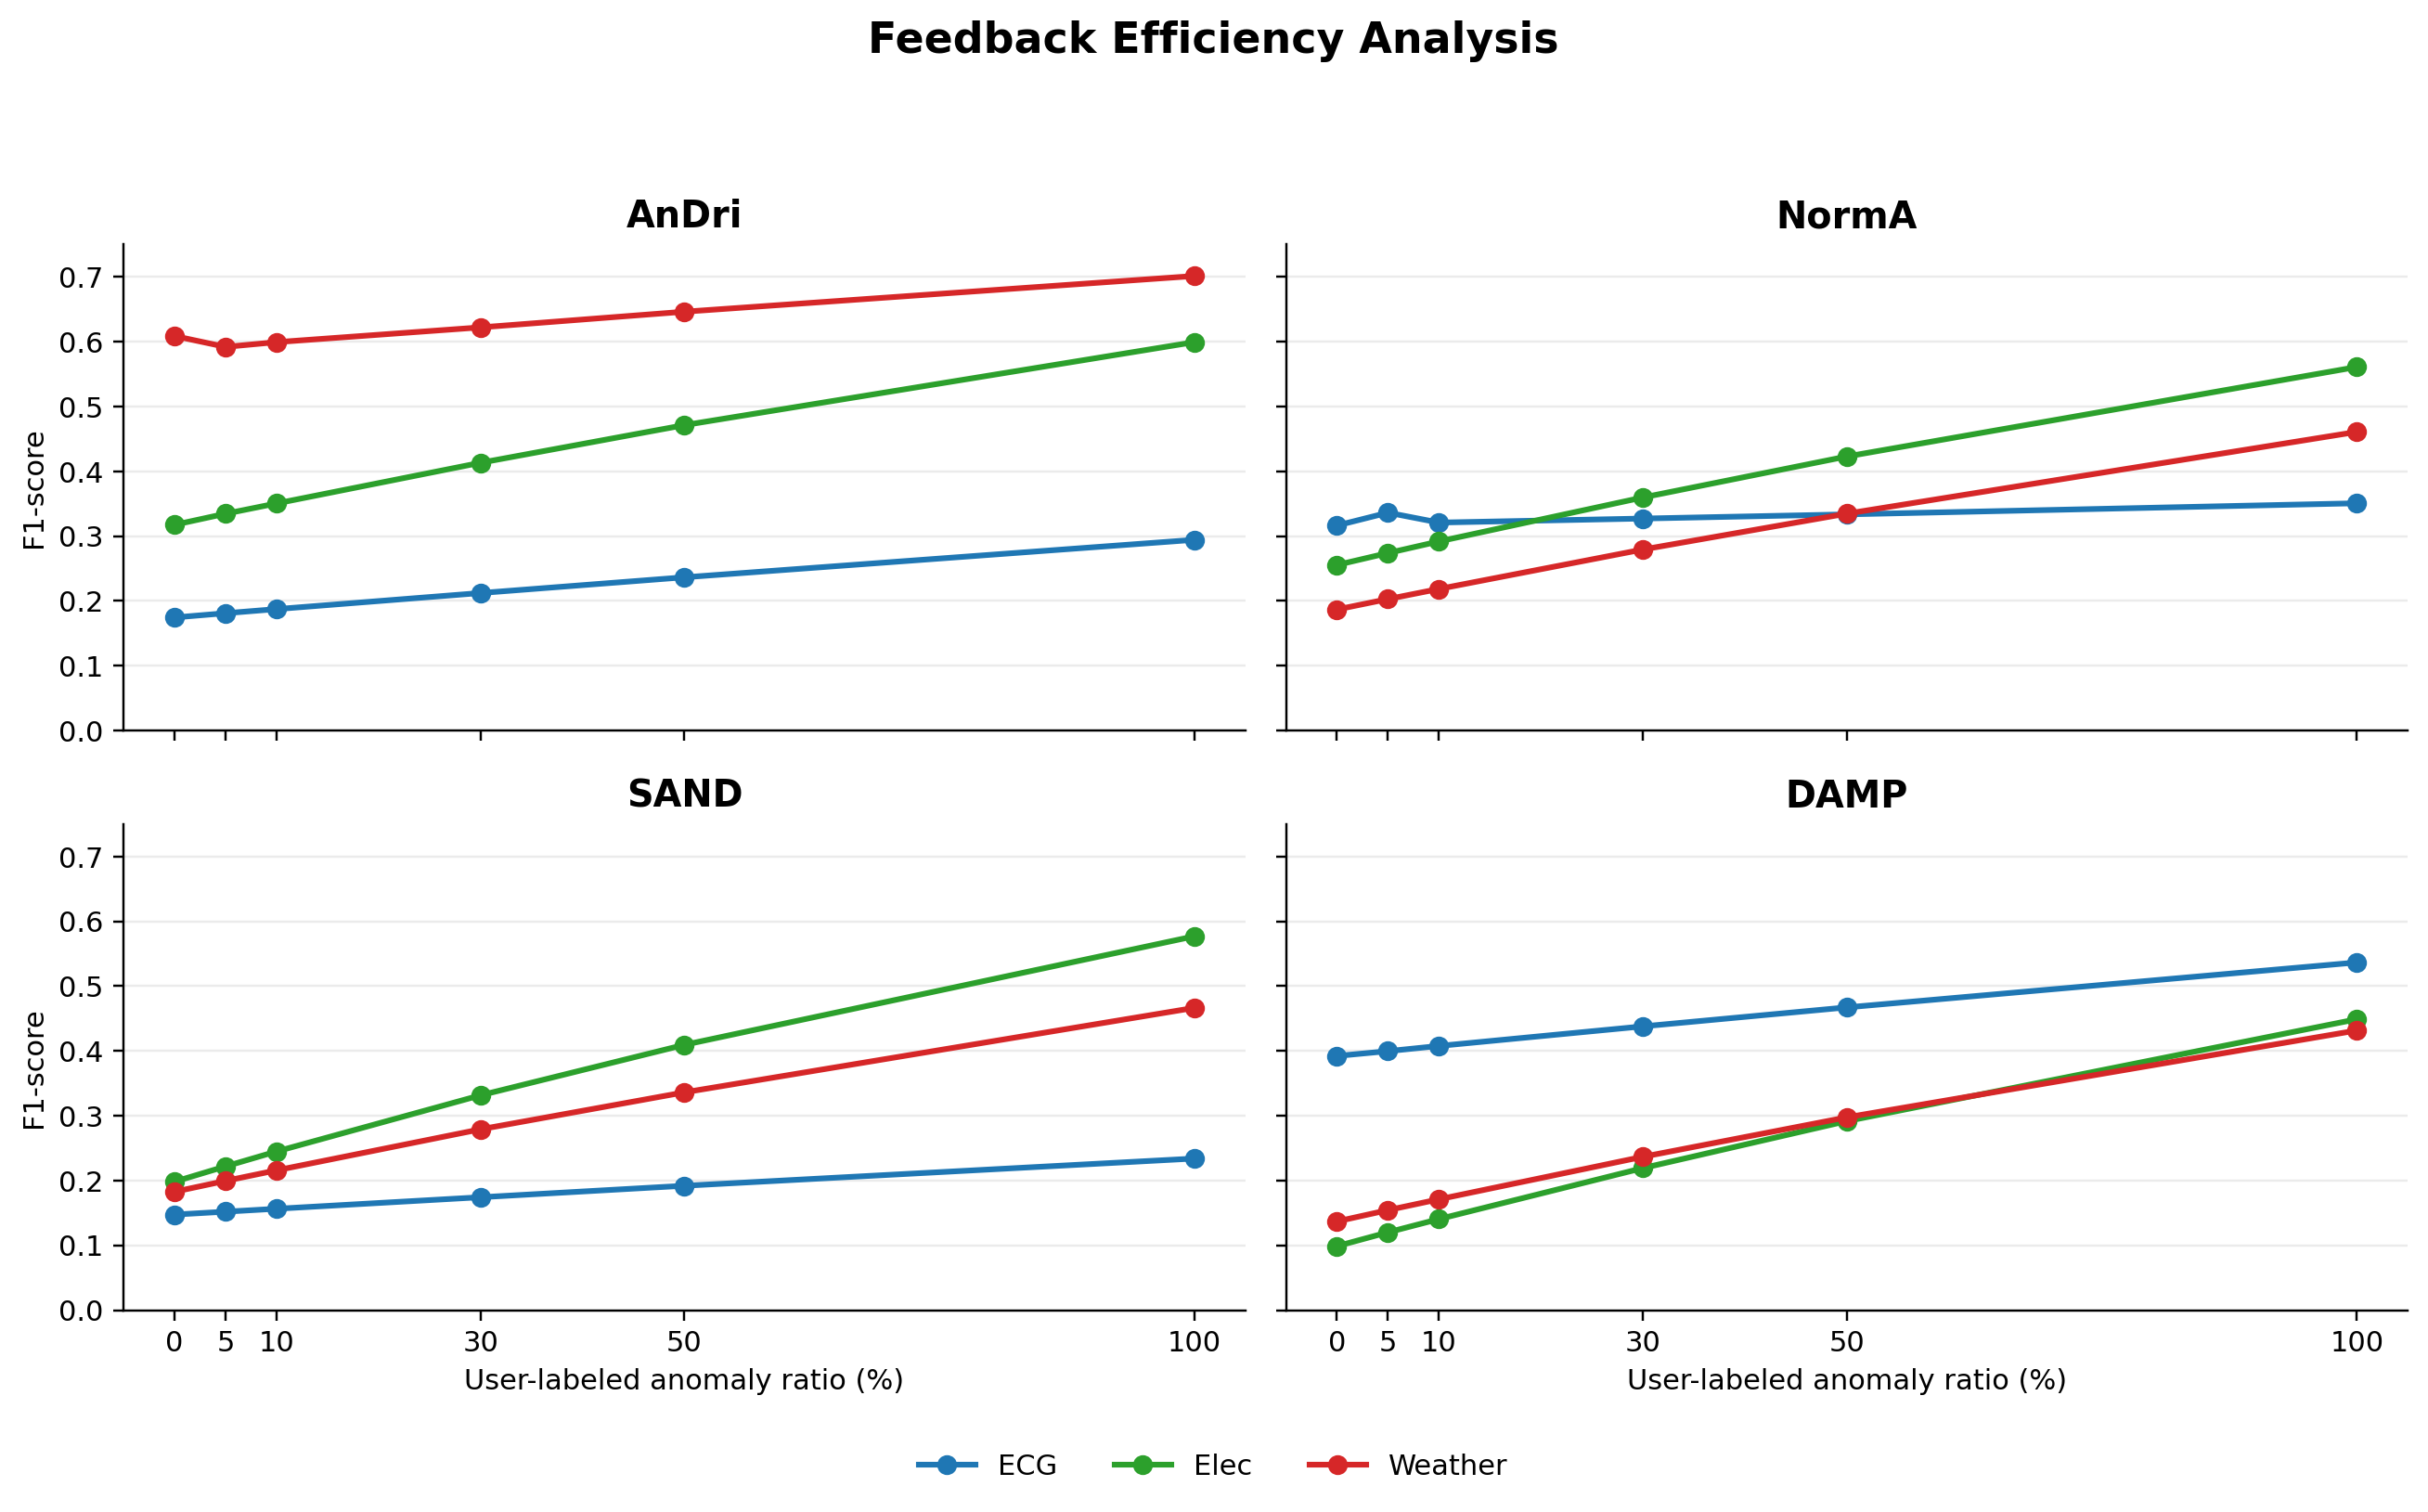
\includegraphics[width=\textwidth]{figures/feedback_efficiency_f1_curves.png}
\caption{Feedback efficiency analysis under different user-labeled anomaly ratios.}
\label{fig:63}
\end{figure}

Figure~\ref{fig:63} shows that the F1-score generally increases as more anomaly labels become available. 

This trend is particularly evident on the Elec dataset. As the proportion of abnormal annotations by users increases, all four methods show a continuous improvement. Similar changes were observed on the ECG and Weather datasets, but the improvement was smaller. In the Weather dataset, Andri was able to achieve relatively strong performance even with limited feedback, so the improvement process was gradual. In the ECG dataset, the lower abnormal ratio (5\%) led to fewer abnormal labels for threshold optimization, which might have limited the impact of additional feedback. Overall, the results indicate that useful improvements can be achieved even with partial user feedback.



\subsection{Discussion and Limitations}

The observed performance improvement is consistent with the design of the threshold-refinement process. As more anomaly labels are provided, the system gains a better understanding of the anomaly-score distribution and can estimate a more appropriate decision threshold. Consequently, the final anomaly labels become more accurate.

Another observation is that the feedback mechanism is beneficial not only to AnDri but also to the benchmark method. This indicates that the process is not dependent on a specific anomaly detection algorithm. As long as a method can generate abnormal scores, user feedback can be incorporated to improve the conversion process between scores and labels.

However, the user feedback is simulated using real labels, so it is assumed that all provided labels are correct. In practical applications, users may provide incomplete or inaccurate feedback, which may reduce the effectiveness of the optimization process. Future research can explore more realistic user behaviors and study the impact of different active learning strategies on the quality of threshold optimization. Overall, the experimental results show that integrating user feedback into the threshold optimization process can improve anomaly detection performance. 


\section{Visual Anomaly and Drift Co-Exploration Results}

The second group of experiments evaluates the visualization contribution of the AnomDrift. This section shows that the interface can make the behavior of AnDri interpretable. The quantitative results are reported in Table~\ref{tab:t1}, while the figures show the local time-series values, anomaly-score curves, thresholds, and highlighted regions.

\begin{table}[H]
\centering
\small
\caption{Comparative accuracy for the ECG and Weather visual case studies. \citep{park2025andri}.}
\label{tab:t1}
\begin{tabular}{llcccc}
\hline
Dataset & Algorithm & Precision & Recall & F1-Score & AUC \\
\hline
ECG & AnDri & 0.412 & \textbf{0.808} & \textbf{0.546} & \textbf{0.964} \\
ECG & NormA & \textbf{0.679} & 0.391 & 0.496 & 0.887 \\
ECG & SAND  & 0.236 & 0.023 & 0.042 & 0.853 \\
ECG & DAMP  & 0.239 & 0.776 & 0.365 & 0.816 \\
\hline
Weather & AnDri & \textbf{0.50} & 0.57 & \textbf{0.54} & \textbf{0.87} \\
Weather & NormA & 0.19 & 0.40 & 0.25 & 0.63 \\
Weather & SAND  & 0.15 & 0.44 & 0.23 & 0.60 \\
Weather & DAMP  & 0.14 & \textbf{0.77} & 0.23 & 0.66 \\
\hline
\end{tabular}
\end{table}

Table~\ref{tab:t1} shows that AnDri achieves the highest F1-score and AUC on both datasets. On ECG, AnDri also obtains the highest recall, indicating that it detects most of the labelled anomalous ECG points. On Weather, DAMP has the highest recall, but its precision and F1-score are much lower, suggesting that it detects more points as anomalies but also introduces more false positives. In contrast, AnDri provides a better balance between precision and recall.

\subsection{ECG Case Study}

\begin{figure}[H]
    \centering

    \begin{subfigure}{0.75\textwidth}
        \centering
        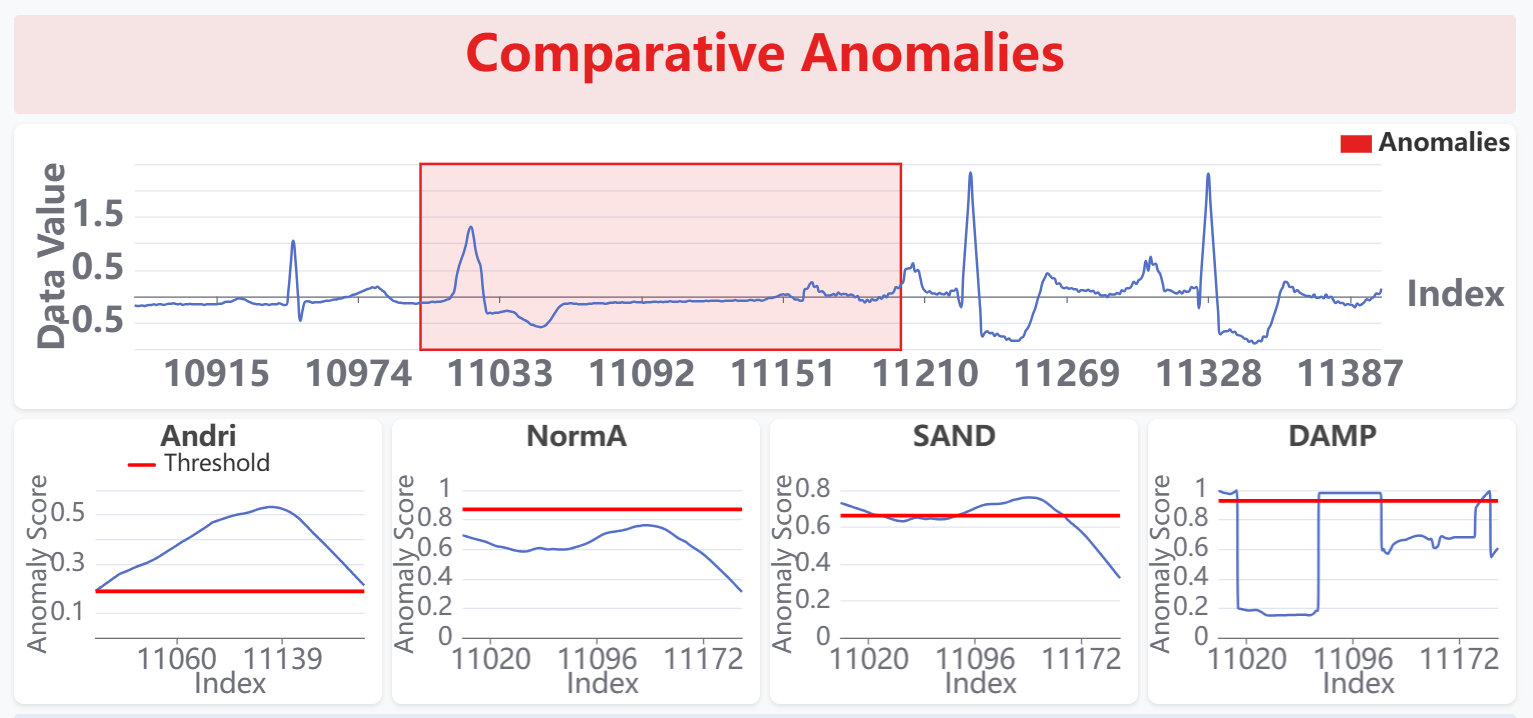
\includegraphics[width=\linewidth]{figures/andri_result1.png}
        \caption{ECG visual comparison of anomalies.}
        \label{fig:66a}
    \end{subfigure}f

    \vspace{0.8em}

    \begin{subfigure}{0.75\textwidth}
        \centering
        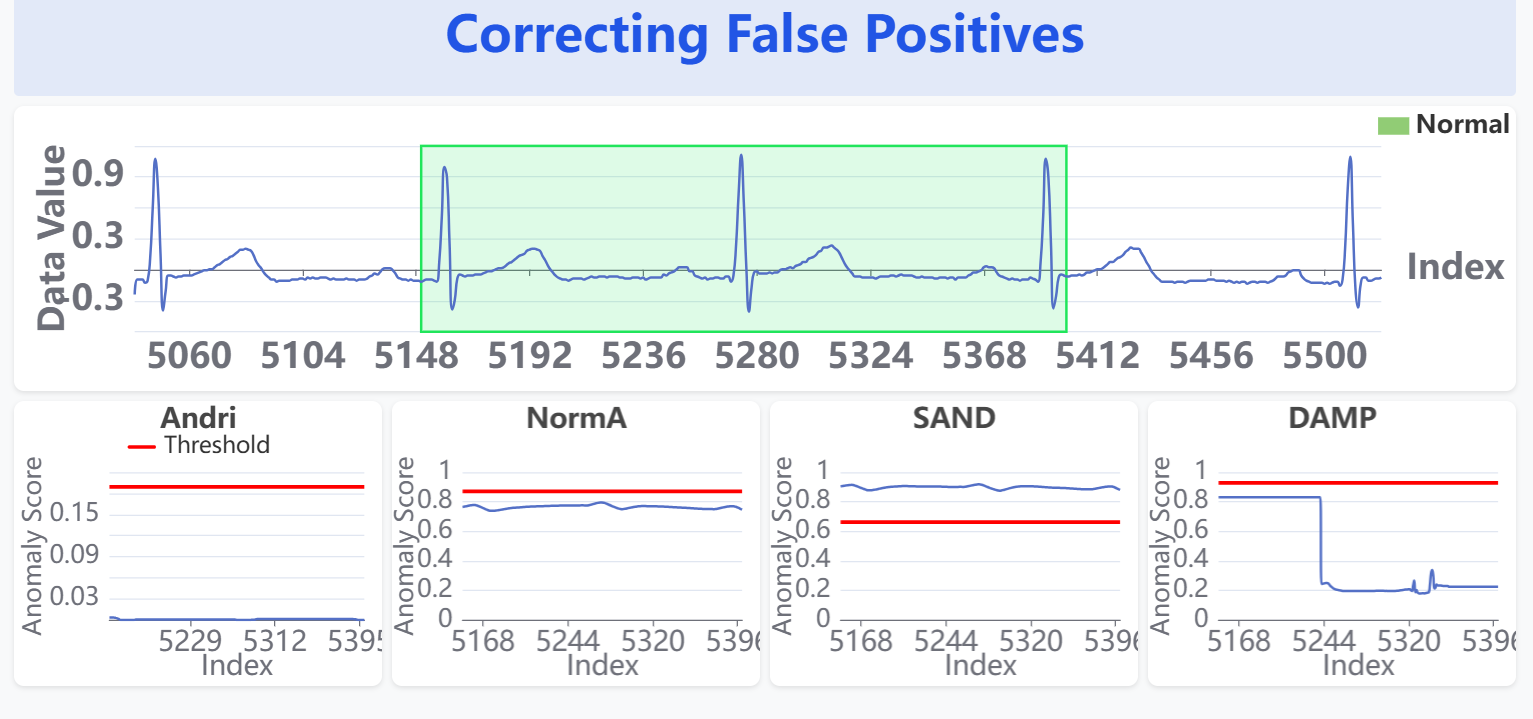
\includegraphics[width=\linewidth]{figures/andri_result2.png}
        \caption{ECG visual comparison of false positives.}
        \label{fig:66b}
    \end{subfigure}
    \caption{}
    \label{fig:66}
\end{figure}


Figure~\ref{fig:66} gives a visual explanation of the ECG results. The top part, labelled ``Comparative Anomalies'', shows a region containing true anomalies. In this region, AnDri's anomaly scores are above its threshold, so the system correctly identifies the region as anomalous. In contrast, NormA and SAND do not clearly separate the anomalous region from normal behavior, which explains their weaker recall.


\fei{Please re-label your figures (a), (b) for more specific references in the text; remove "bottom part" references throughout this section.}

\reply{Divide the image into two sub-figures, remove unclear words 'top' and 'bottom'. Use sub-figures, and use sub-figure 'ref' to replace those unclear words}{Figure~\ref{fig:66} gives a visual explanation of the ECG results. Figure~\ref{fig:66a}, labelled ``Comparative Anomalies'', shows a region containing true anomalies. In this region, AnDri's anomaly scores are above its threshold, so the system correctly identifies the region as anomalous. In contrast, NormA and SAND do not clearly separate the anomalous region from normal behavior, which explains their weaker recall.}
\textcolor{blue}{Figure~\ref{fig:66b}, labelled ``Correcting False Positives'', shows the opposite situation. The highlighted green region represents a change in normal ECG pattern, namely concept drift, rather than true anomaly points. AnDri assigns this region a score below its threshold and correctly treats it as normal behavior under drift. However, the baseline methods produce scores close to or above their thresholds, which can cause them to classify the drift region as anomalous.}

The bottom part, labelled ``Correcting False Positives'', shows the opposite situation. The highlighted green region represents a change in normal ECG pattern, namely concept drift, rather than true anomaly points. AnDri assigns this region a score below its threshold and correctly treats it as normal behavior under drift. However, the baseline methods produce scores close to or above their thresholds, which can cause them to classify the drift region as anomalous.

\subsection{Weather Case Study}

\begin{figure}[H]
    \centering

    \begin{subfigure}{0.75\textwidth}
        \centering
        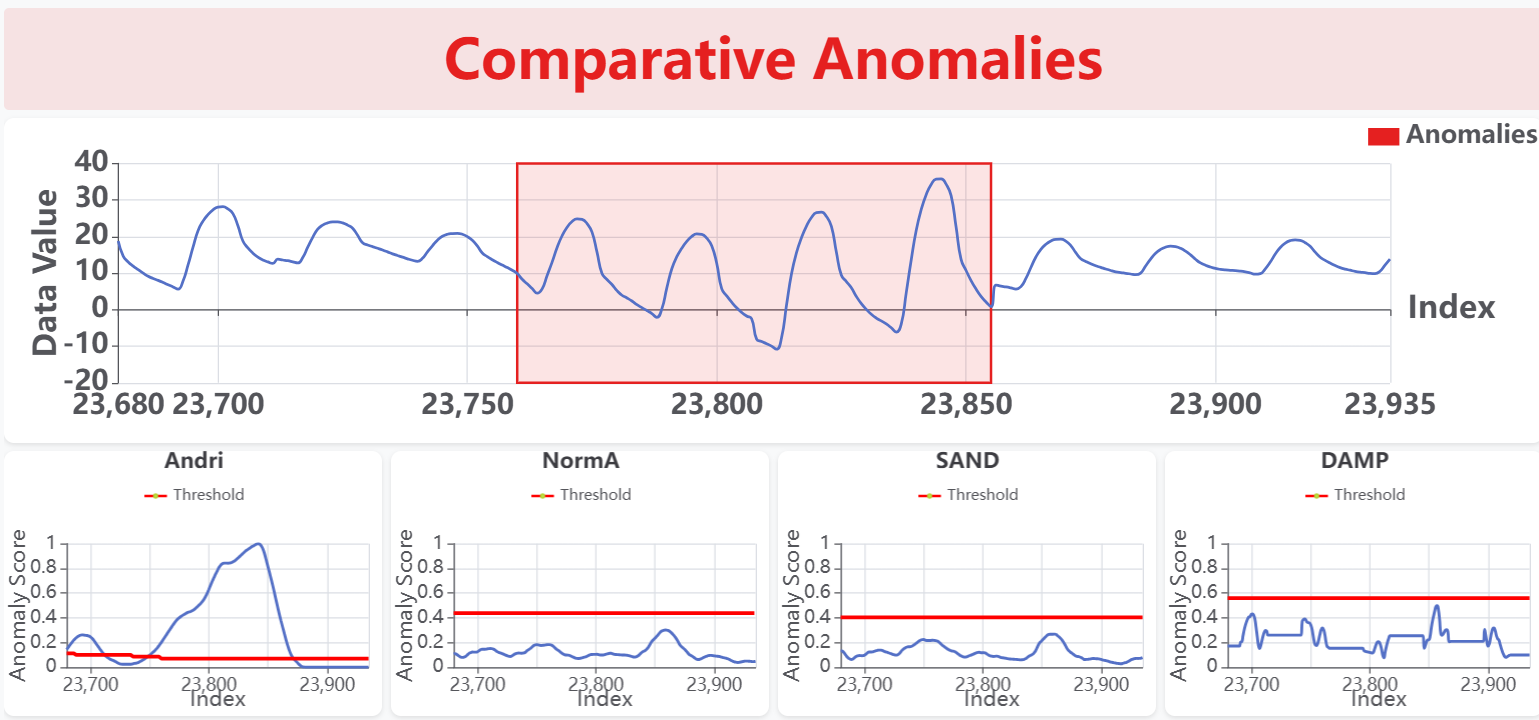
\includegraphics[width=\linewidth]{figures/weather1.png}
        \caption{Weather visual comparison of anomalies.}
        \label{fig:65a}
    \end{subfigure}f

    \vspace{0.8em}

    \begin{subfigure}{0.75\textwidth}
        \centering
        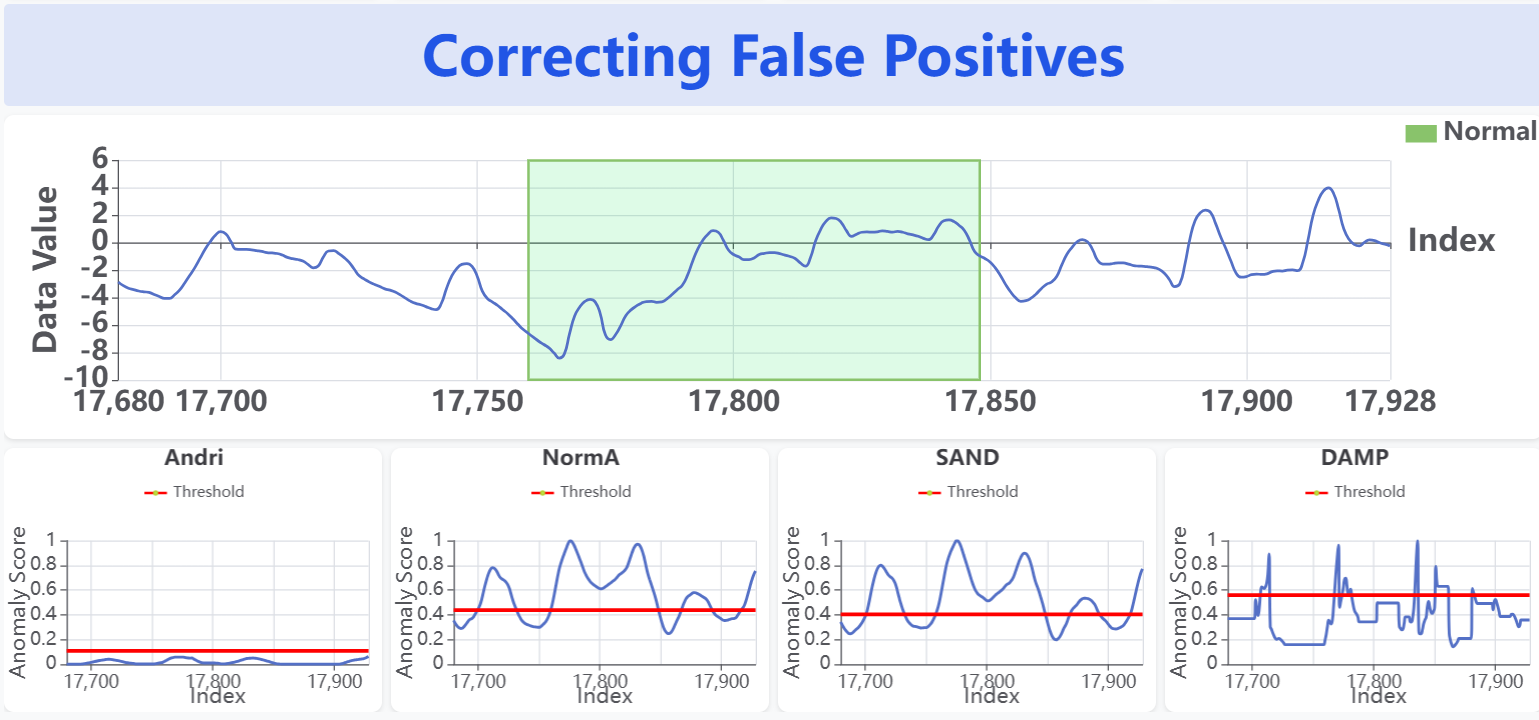
\includegraphics[width=\linewidth]{figures/weather2.png}
        \caption{Weather visual comparison of false positives.}
        \label{fig:65b}
    \end{subfigure}
    \caption{}
    \label{fig:65}
\end{figure}

\reply{Divide the image into two sub-figures, remove unclear words 'top' and 'bottom'. Use sub-figures, and use sub-figure 'ref' to replace those unclear words}{Figure~\ref{fig:65} provides an additional example on the Weather dataset. Similar to the ECG case, figure~\ref{fig:65a} shows a true anomaly interval highlighted in red. In this region, AnDri's score rises above its threshold, while the scores of NormA, SAND, and DAMP remain below their thresholds. This indicates that AnDri detects the anomalous interval, whereas the baseline methods miss it.}

\textcolor{blue}{Figure~~\ref{fig:65b} shows a normal interval highlighted in green. AnDri keeps its score below the threshold and correctly treats the region as normal. In contrast, the baseline methods produce higher scores and may classify parts of this normal region as anomalies. This example shows that the same visualization design can also explain AnDri's behaviour on the Weather dataset, where seasonal variation and gradual drift make anomaly detection challenging.}

Figure~\ref{fig:65} provides an additional example on the Weather dataset. Similar to the ECG case, the top part shows a true anomaly interval highlighted in red. In this region, AnDri's score rises above its threshold, while the scores of NormA, SAND, and DAMP remain below their thresholds. This indicates that AnDri detects the anomalous interval, whereas the baseline methods miss it.

The bottom part shows a normal interval highlighted in green. AnDri keeps its score below the threshold and correctly treats the region as normal. In contrast, the baseline methods produce higher scores and may classify parts of this normal region as anomalies. This example shows that the same visualization design can also explain AnDri's behaviour on the Weather dataset, where seasonal variation and gradual drift make anomaly detection challenging.